\documentclass[a4paper, 12pt]{article}

\def\languages{french, english}

%%%%%%%%%%%%%%%%%%% Packages

%%%%% Tools

\usepackage{comment}
\usepackage{lipsum}
\usepackage{xstring}

%%%%% Document

\usepackage[pdfusetitle]{hyperref}

\usepackage{geometry}
\geometry{paper=a4paper,top=3.5cm,bottom=2.5cm,right=2.5cm,left=2.5cm}

\usepackage{fancyhdr}
%\pagestyle{fancy}
%\fancyhead[L]{}
%\fancyhead[R]{\leftmark}
%\fancyfoot[C]{\thepage}
%\renewcommand{\headrulewidth}{0pt}

%%%%% Text

\usepackage[utf8]{inputenc}
\usepackage[T1]{fontenc}
\edef\restoreparindent{\parindent=\the\parindent\relax}
\usepackage[parfill]{parskip}
%\restoreparindent
\usepackage{csquotes}

\newlength{\mytextsize}
\makeatletter
\setlength{\mytextsize}{\f@size pt}
\makeatother

%%%%% Languages

\ifx\languages\undefined
	\usepackage[english]{babel}
\else
	\usepackage[\languages]{babel}
\fi

% english

\addto\captionsenglish{\def\figurename{Figure}}
\addto\captionsenglish{\def\tablename{Table}}

\def\st{\text{s.t.}}

% french

\frenchbsetup{StandardLists=true}

\addto\captionsfrench{\def\figurename{Figure}}
\addto\captionsfrench{\def\tablename{Table}}
\addto\captionsfrench{\def\proofname{Preuve}}

\def\tq{\text{t.q.}}
\def\cad{c.-à-d.}
\def\Cad{C.-à-d.}

%%%%% Styles

\usepackage[skip=\mytextsize]{caption}
\usepackage{float}
\usepackage{mdframed}
\usepackage{enumitem}
\usepackage{eurosym}
\usepackage{color}

\newcommand\caaption[1]{\caption{#1}\vspace{-1\mytextsize}}

%%%%% Mathematics

\usepackage{amsmath}
\usepackage{amssymb}
\usepackage{amsfonts}
\usepackage{bm}
\usepackage{esint}
\usepackage[makeroom]{cancel}

\newcommand{\fact}[1]{#1!}
\newcommand{\e}[1]{\mathbf{e}_{#1}}
\newcommand{\deriv}{\mathrm{d}}
\DeclareMathOperator{\tr}{tr}


%%%%% SI units

\usepackage[squaren,Gray,cdot]{SIunits}
\usepackage{sistyle}

\IfStrEq{\languagename}{french}{
	\SIdecimalsign{,}
}

%%%%% Chemistry

\usepackage[version=4]{mhchem}

%%%%% Table & Figure

\usepackage{array}
\usepackage{tabularx}
\usepackage{multirow}
\usepackage{multicol}
\newcolumntype{M}[1]{>{\centering\arraybackslash}m{#1}}
%\setlength\extrarowheight{0em}
\renewcommand{\arraystretch}{1.3}

\usepackage{pgfplots}
\usepackage{tikz}
\usetikzlibrary{shapes.geometric, positioning}
\usepackage{graphics}
\usepackage{graphicx}
\pgfplotsset{axis on top, compat = 1.3}

%%%%%% Theorems and Definitions

\usepackage{amsthm}
\usepackage{thmtools}

\def\lgthm{Theorem}
\def\lglem{Lemma}
\def\lgprop{Proposition}
\def\lgdefn{Definition}
\def\lghyp{Hypothesis}
\def\lgquest{Question}
\def\lgansw{Answer}
\def\lgexpl{Example}
\def\lgrmk{Remark}
\def\lgnote{Note}
\def\lgtip{Tip}

\IfStrEq{\languagename}{french}{
	\def\lgthm{Théorème}
	\def\lglem{Lemme}
	\def\lgprop{Proposition}
	\def\lgdefn{Définition}
	\def\lghyp{Hypothèse}
	\def\lgquest{Question}
	\def\lgansw{Réponse}
	\def\lgexpl{Exemple}
	\def\lgrmk{Remarque}
	\def\lgnote{Note}
	\def\lgtip{Conseil}
}

\theoremstyle{plain}
\newtheorem{thm}{\lgthm}[section]
\newtheorem{lem}{\lglem}[section]
\newtheorem{prop}{\lgprop}[section]

\theoremstyle{definition}
\newtheorem{defn}{\lgdefn}[section]
\newtheorem{hyp}{\lghyp}[section]
\newtheorem{quest}{\lgquest}[]

\declaretheorem[
name=\lgansw,
qed={\lower-0.3ex\hbox{$\triangle$}},
within=quest
]{answ}

\declaretheorem[
name=\lgexpl,
qed={\lower-0.3ex\hbox{$\triangle$}},
within=section
]{expl}

\theoremstyle{remark}
\newtheorem*{rmk}{\lgrmk}
\newtheorem*{note}{\lgnote}
\newtheorem*{tip}{\lgtip}

\begingroup
\makeatletter
\@for\theoremstyle:=definition,remark,plain\do{%
	\expandafter\g@addto@macro\csname th@\theoremstyle\endcsname{%
		\addtolength\thm@preskip\parskip
	}%
}
\endgroup

%%%% Others

\renewcommand{\qedsymbol}{$\blacksquare$}

\newcommand{\mytableofcontents}{
	\newpage
	\pagenumbering{roman}
	\tableofcontents
	\newpage
	\pagenumbering{arabic}
}

%%%%%%%%%%%%%%%%%%%
%%%% Code

\usepackage{xcolor}
\usepackage{listings}

\definecolor{jblue}{rgb}{0.13,0.13,1}
\definecolor{jgreen}{rgb}{0,0.5,0}
\definecolor{jred}{rgb}{0.9,0,0}

\definecolor{cgreen}{rgb}{0,0.6,0}
\definecolor{cgray}{rgb}{0.5,0.5,0.5}
\definecolor{cpurple}{rgb}{0.58,0,0.82}
\definecolor{cbackground}{rgb}{0.95,0.95,0.92}

\lstdefinestyle{MyC}{
	language=C,
	%%%%%%
	showstringspaces=false,
	extendedchars=true,
	tabsize=4,
	columns=fixed,
	%%%%%%
	breaklines=true,
	breakatwhitespace=true,
	prebreak=\space,
	%%%%%%
	basicstyle=\footnotesize\fontfamily{pcr},
	keywordstyle=\color{magenta},
	commentstyle=\itshape\color{cgreen},
	stringstyle=\color{cpurple},
	%%%%%%
	numbersep=0.5\mytextsize,
	numbers=left,
	numberstyle=\tiny\color{cgray},
	%%%%%%
	frame=single,
	backgroundcolor=\color{cbackground},
	rulecolor=\color{black},
	framexleftmargin=2\mytextsize,
	xleftmargin=2\mytextsize,
	captionpos=b,
	%%%%%%
	aboveskip=1.5em
}

\lstset{emph = {shared, memory, semaphore, semaphores, worker, workers, master, masters, message, messages, queue, queues, chan, signal, wait, ?, !}, emphstyle = {\color{black}\bfseries}}

\lstdefinestyle{MyJava}{
	language=Java,
	%%%%%%
	showstringspaces=false,
	extendedchars=true,
	tabsize=4,
	columns=fixed,
	%%%%%%
	breaklines=true,
	breakatwhitespace=true,
	prebreak=\space,
	%%%%%%
	basicstyle=\footnotesize\ttfamily,
	keywordstyle=\color{jblue},
	commentstyle=\color{jgreen},
	stringstyle=\color{jred},
	%%%%%%
	numbersep=0.2\mytextsize,
	numbers=left,
	numberstyle={\ttfamily\footnotesize},
	%%%%%%
	frame=single,
	rulecolor=\color{black},
	framexleftmargin=2\mytextsize,
	xleftmargin=2\mytextsize,
	captionpos=b
}

\lstdefinestyle{MyMatlab}{
	language=Matlab,
	%%%%%%
	showstringspaces=false,
	extendedchars=true,
	tabsize=4,
	columns=fixed,
	%%%%%%
	breaklines=true,
	breakatwhitespace=true,
	prebreak=\space,
	%%%%%%
	basicstyle=\footnotesize\fontfamily{pcr},
	keywordstyle=\color[rgb]{0,0,1},
	commentstyle=\itshape\color{green!40!black},
	stringstyle=\color[rgb]{.627,.126,.941},
	%%%%%%
	numbersep=0.5\mytextsize,
	numbers=left,
	numberstyle={\lstbasicfont\footnotesize},
	%%%%%%
	frame=single,
	rulecolor=\color{black},
	framexleftmargin=2\mytextsize,
	xleftmargin=2\mytextsize,
	captionpos=b
}

\lstdefinestyle{MyVHDL}{
	language=VHDL,
	%%%%%%
	showstringspaces=false,
	extendedchars=true,
	tabsize=4,
	columns=fixed,
	%%%%%%
	breaklines=true,
	breakatwhitespace=true,
	prebreak=\space,
	%%%%%%
	basicstyle=\footnotesize\ttfamily,
	keywordstyle=\color{blue!100!black!80},
	commentstyle=\itshape\color{green!90!black!90},
	stringstyle=\color[rgb]{.627,.126,.941},
	%%%%%%
	numbersep=0.5\mytextsize,
	numbers=left,
	numberstyle={\footnotesize},
	%%%%%%
	frame=single,
	rulecolor=\color{black},
	framexleftmargin=2\mytextsize,
	xleftmargin=2\mytextsize,
	captionpos=b
}

\usepackage{clrscode3e}
\makeatletter
\AtBeginDocument{
	\hypersetup{
		pdftitle={\@title},
		pdfauthor={Maxime Meurisse, Valentin Vermeylen},
		pdfkeywords={maxime, meurisse, valentin, vermeylen, university, liege, radix, sort, parallel, computing, computation, structures, latex, document},
		pdfproducer={LaTeX document},
		pdfcreator={Document generated with pdflatex}
	}
}

%%%%%%%%%%%%%%%%%%% Titlepage

\def\logopath{resources/pdf/logo-uliege.pdf}
\def\toptitle{Computation structures}
\title{Radix sort}
\def\subtitle{Project 2 - Parallel programming}
%\def\authorhead{Authors}
\author{Maxime \textsc{Meurisse} (20161278)\\Valentin \textsc{Vermeylen} (20162864)\\}
%\def\rightauthorhead{}
%\def\rightauthor{}
\def\context{University of Liège}
\date{Academic year 2018-2019}

%%%%%%%%%%%%%%%%%%%

\begin{document}
    % ---------- Title page ---------- %
	\newgeometry{margin = 2.5cm}
\makeatletter
\begin{titlepage}
	\begin{minipage}[t][0.425\textheight][t]{\textwidth}
		\begin{center}
		    \ifx\toptitle\undefined
    		    \vfill
    		    \ifx\logopath\undefined
    		    \else
    			    \includegraphics[height=0.2125\textheight]{\logopath}
    			\fi
    		\else
    		    \ifx\logopath\undefined
    		    \else
    			    \includegraphics[height=0.15\textheight]{\logopath}
    			\fi
    			\vfill
    			{\huge \textsc{\toptitle}}
			\fi
			\vfill
		\end{center}
	\end{minipage}
	\vfill
	\begin{minipage}{\textwidth}
		\hspace{0.5em}
		\begin{mdframed}[linewidth = 2pt, innertopmargin = 1em, innerbottommargin = 1em, leftline = false, rightline = false]
			\begin{center}
				{\huge \bfseries \@title}
			\end{center}
		\end{mdframed}
		\hspace{0.5em}
	\end{minipage}
	\vfill
	\begin{minipage}[b][0.425\textheight][t]{\textwidth}
			\ifx\subtitle\undefined
			\else
			    \vspace{-0.5em}
			    \begin{center}
				    {\LARGE \subtitle}
				\end{center}
			\fi
			\vfill
			\ifx\rightauthor\undefined
			    \begin{center}
			        \ifx\authorhead\undefined
			        \else
		                {\large\it \authorhead\\[0.5em]}
		            \fi
			        {\large \@author}
			    \end{center}
			\else
			    \begin{minipage}[t]{0.5\textwidth}
			        \begin{flushleft}
			            \ifx\authorhead\undefined
			            \else
			                {\large\it \authorhead\\[0.5em]}
			            \fi
				        {\large \@author}
				    \end{flushleft}
				\end{minipage}
				\begin{minipage}[t]{0.5\textwidth}
				    \begin{flushright}
				        \ifx\rightauthorhead\undefined
			            \else
			                {\large\it \rightauthorhead\\[0.5em]}
			            \fi
				        {\large \rightauthor}
				    \end{flushright}
				\end{minipage}
			\fi
			\vfill
			\begin{center}
			    \ifx\context\undefined
			    \else
			        {\large \context \\[0.5em]}
			    \fi
			    {\large \@date}
			\end{center}
	\end{minipage}
\end{titlepage}
\makeatother
\restoregeometry
	
	
	% ---------- Presentation ---------- %
	\section{Presentation}
	The goal of this project is to implement the \og radix sort\fg{} sorting algorithm (for positive integer arrays) using parallel programming mechanisms.\par
	
	To this end, several files have been created:
	
	\begin{itemize}
	    \item \texttt{array.c}: a personal library containing functions useful for manipulating arrays, and more specifically the implementation of two-dimensional arrays in one-dimensional arrays;
	    \item \texttt{communication.c}: a personal library containing a series of functions allowing easier manipulation of parallel programming mechanisms with \href{https://fr.wikipedia.org/wiki/UNIX_System_V}{System V};
	    \item \texttt{main.c}: the main file of the project. It retrieves the data entered by the user and contains the implementation of the sorting algorithm as well as all the parallel programming mechanisms.
	\end{itemize}
	
	The project was compiled on the student machines of the Montefiore Institute thanks to the following command: \texttt{gcc main.c array.c communication.c -{}-pedantic -Wall -Wextra -Wmissing-prototypes -lm -o main}.\par
	
	The algorithm can then be called via the command: \texttt{./main (base) (size) (numbers)}. For example, the command \texttt{./main 10 4 54 23 6 12} will sort the array \texttt{[54, 23, 6, 12]} of size \texttt{4} whose elements are in base \texttt{10}.
	
	
	% ---------- Implementation ---------- %
	\section{Implementation}
	
	\subsection{Parallel programming mechanisms}
	
	\subsubsection{Shared memory}
	Several pieces of information have been placed in the shared memory:
	
	\begin{itemize}
	    \item \texttt{numbers[]}: it is the main array containing the numbers to sort. This one is placed in the shared memory because all the worker must read and write in it;
	    \item \texttt{temp[]}: this is the two-dimensional temporary array (but we decided to concatenate it in a one-dimensional array) to store the elements for sorting. It is placed in shared memory because all workers must write and read in it;
	    \item \texttt{sorted}: this variable is used to tell each worker whether the array is sorted or not. It is placed in shared memory because all workers must be able to read it and the master must be able to modify it. Note that, if it's modified by the master, the workers do not have access to it thanks to semaphore waiting.
	\end{itemize}
	
	The shared memory is presented in the listing \ref{lst:shared}.\par
	
	\lstinputlisting[style={MyC}, caption={Shared memory.}, label={lst:shared}]{resources/c/shared.c}
	
	\subsubsection{Semaphores}
	In order to ensure mutual exclusion, several semaphores are used:
	
	\begin{itemize}
	    \item \texttt{worker}: this semaphore is used to check that all the workers have finished their work (first the writing phase of the main array to the temporary array, then the writing phase of the temporary array to the main array) before the master continues his execution;
	    \item \texttt{master}: this is a set of 2 semaphores. These semaphores are used so that workers wait for the master to complete its calculations before re-writing the contents of the temporary array to the main array. They also ensure that we do not try to read from something that is currently being updated.
	\end{itemize}
	
	These semaphores are presented in the listing \ref{lst:semaphores}.\par
	
	\lstinputlisting[style={MyC}, caption={Semaphores.}, label={lst:semaphores}]{resources/c/semaphore.c}
	
	\subsubsection{Message queues}
	We decided to use two message queues, presented in the listing \ref{lst:msgq}, to exchange messages between the master process and the workers. Each process will fill it with its \texttt{digit + 1} as \texttt{mtype}, to ensure the message will reach the right recipient, and an array containing the digit used and the position to start writing in the main array, or the number of numbers on a given line in the temporary array depending on the sender (namely master and worker).\par
	
	To summarize and make it clearer, here is the content of each queue: 
	
	\begin{itemize}
	    \item worker to master: \texttt{(id + 1, [digit, numbers])};
	    \item master to worker: \texttt{(id + 1, [pos])}.
	\end{itemize}
	
	\paragraph{Remark} We used \texttt{id + 1} as \texttt{mtype} must be positive and we didn't want to use 0 for worker 0 by fear of unexpected results.\par
	
	\lstinputlisting[style={MyC}, caption={Message queues.}, label={lst:msgq}]{resources/c/chan.c}
	
	\subsubsection{Processes}
	The main process \texttt{main}, presented in the listing \ref{lst:main}, is in charge of getting the arguments passed as parameters to the program, creating the IPC elements, creating the different processes that will sort the array and finally displaying the sorted array.\par
	
	\lstinputlisting[style={MyC}, caption={Main process.}, label={lst:main}]{resources/c/main.c}
	
	The program, in addition to this main process, uses 2 different processes:
	
	\begin{itemize}
	    \item \texttt{worker}: there are as many worker as the base. Each worker first deals with placing some numbers in the temporary array, and secondly re-writing those numbers in the final array. Each of these operations involves communication with the master process;
	    \item \texttt{master}: there is only one master process. The first task is to receive the information of each worker about the number of numbers in each line of the temporary array. It then takes care of communicating to each worker the position at which he can begin to rewrite in the final array. Once that is done, it resets the temporary array to -1 everywhere.
	\end{itemize}
	
	These processes are presented in the listings \ref{lst:worker} and \ref{lst:master}.\par
	
	\lstinputlisting[style={MyC}, caption={Process \texttt{worker}.}, label={lst:worker}]{resources/c/worker.c}
	\lstinputlisting[style={MyC}, caption={Process \texttt{master}.}, label={lst:master}]{resources/c/master.c}
	
	\subsection{Sorting procedure}
	The sorting of the array is done in several stages with the elements presented previously.
	
	\begin{enumerate}
	    \item First, after creating all the processes, each worker takes care of reading a part of the array containing the numbers to sort. Each worker reads a different part (if the base is greater than the size of the array, some workers should not do anything during this step). There is therefore no conflict between the workers during the reading. The bounds in which they read are \texttt{begin} and \texttt{end} in the listing \ref{lst:worker}.
	    \item Secondly, and immediately after reading, each worker places his read items in the temporary array according to the digit (therefore the iteration) concerned. Each worker writes the element to the line corresponding to its \texttt{id} and in the column corresponding to the position of the element read in the array. It is therefore impossible for many workers to write a number in the same place in the temporary array and we do not need semaphore to restrict access to the array. Each number is correctly sorted in that array. After this step, a semaphore is used to wait for each worker to finish writing before proceeding to the next step. The master then indicates that each worker can proceed to the next step with another semaphore (\texttt{sem\_master[0]}).
	    \item Thirdly, each worker calculates the number of elements on the line of the temporary array he is dealing with (that is, the number of elements different from -1 on the \texttt{id}\up{th} line of the temporary array). Each worker sends this number of elements to the master via the first message queue with its \texttt{id + 1} as \texttt{mtype}.
	    \item Fourthly, depending on the number of elements on a worker's line, the master calculates from which position in the main array the worker must write back its elements. The master sends each worker his rewrite position via the second message queue. A semaphore is used to wait for each worker to finish writing his items before moving on.
	    \item Finally, depending on the current iteration, either the temporary array is reset and it moves to the next iteration, or it was the last iteration and the array is sorted. In this case, the workers are told via the sorted variable that the sort is complete. A semaphore (\texttt{sem\_master[1]}) is used to avoid the workers reading \texttt{sorted} before it is updated if needed.
	    
	    \paragraph{Remark} The last set of semaphore waits is used so that each worker has finished with all memory elements before the master deletes the semaphores, message queues and shared memory segments. That avoids a \og semops: invalid arguments\fg{} as a worker waits for a semaphore that does not exist anymore.
	\end{enumerate}
	
	\subsection{Schematic summary of the communications}
	The communication between the different processes is carried out thanks to the semaphores and the message queue described above. This communication is shown schematically in the figure \ref{fig:communication_processes}.
	
	\begin{figure}[!ht]
	    \centering
	    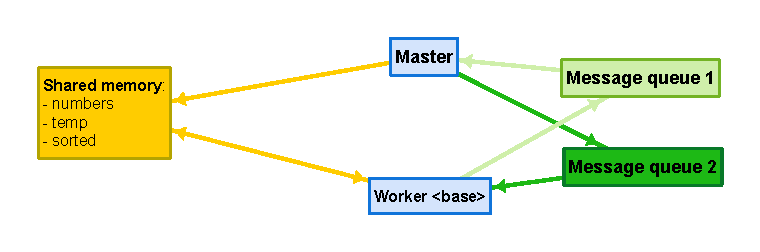
\includegraphics[width=\textwidth]{resources/pdf/communication.pdf}
	    \caption{Schematic representation of the communication between the different processes.}
	    \label{fig:communication_processes}
	\end{figure}
	
	
	% ----- Conclusion ----- %
	\section{Conclusion}
	In conclusion, we can say that a parallel implementation is more difficult to implement than a sequential implementation, but drastically more effective.\par
	
	Indeed, in order to manage the synchronization between the processes and the sharing of the memory elements (which could be shared between several distorted machines), more advanced techniques are required and a particular attention must be paid in order not to have conflicts.\par
	
	However, these parallel programming techniques make it possible to perform a greater number of operations in a much shorter time, and thus to obtain results that could not be obtained via a sequential implementation.\par
	
	Parallel programming is generally used for calculations much larger than those of this project, but it has already allowed us to observe all the effectiveness of parallelism on sorts of arrays containing a large amount of elements.
\end{document}
